\begin{pastexam}[label={px:ncku-114-cce-ds-18}]{成大電通所 114 學年度 簡答題第 2 題}
（簡答）

(10 PTs) Given a graph shown in Fig 2, please answer the following questions:\\
a) which are the articulation points, and\\
b) the biconnected components of the graph.

\begin{center}
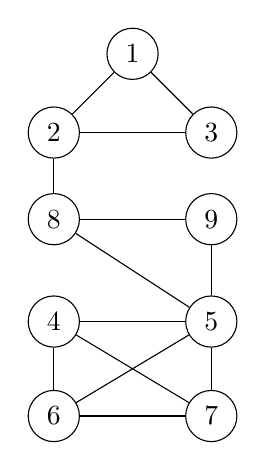
\begin{tikzpicture}[v/.style={circle,draw,inner sep=1pt,minimum size=6.5mm},w/.style={font=\small,inner sep=1.5pt}]
\node[v] (n1) at (1.00,0.00) {1};
\node[v] (n2) at (0.00,-1.00) {2};
\node[v] (n3) at (2.00,-1.00) {3};
\node[v] (n8) at (0.00,-2.10) {8};
\node[v] (n9) at (2.00,-2.10) {9};
\node[v] (n4) at (0.00,-3.40) {4};
\node[v] (n5) at (2.00,-3.40) {5};
\node[v] (n6) at (0.00,-4.60) {6};
\node[v] (n7) at (2.00,-4.60) {7};
\draw[] (n1) -- (n2);
\draw[] (n1) -- (n3);
\draw[] (n2) -- (n3);
\draw[] (n2) -- (n8);
\draw[] (n8) -- (n9);
\draw[] (n8) -- (n5);
\draw[] (n9) -- (n5);
\draw[] (n4) -- (n5);
\draw[] (n4) -- (n6);
\draw[] (n4) -- (n7);
\draw[] (n5) -- (n6);
\draw[] (n5) -- (n7);
\draw[] (n6) -- (n7);
\end{tikzpicture}\\
Fig. 2
\end{center}
\end{pastexam}

\begin{pastsoln}
答案：(a) 割點是 2、5、8。 (b) 雙連通元件有四個：$\{1, 2, 3\}$、$\{2, 8\}$、$\{5, 8, 9\}$、$\{4, 5, 6, 7\}$。

圖的邊：1--2、1--3、2--3、2--8、8--9、8--5、9--5、4--5、4--6、4--7、5--6、5--7、6--7。

\textbf{(a)} 用資結書第~23.5~節的 DFS 加 low 值求割點。 從 1 開始，鄰居依編號由小到大走。 $d[v]$ 是發現的順序，
$\mathit{low}[v]$ 是 $v$ 的子樹經由至多一條後向邊能到的最小 $d$ 值：
\begin{center}
\begin{tabular}{l*{9}{c}}
\toprule
頂點 & 1 & 2 & 3 & 8 & 5 & 4 & 6 & 7 & 9 \\
\midrule
DFS 樹上的父節點 & -- & 1 & 2 & 2 & 8 & 5 & 4 & 6 & 5 \\
$d$ & 1 & 2 & 3 & 4 & 5 & 6 & 7 & 8 & 9 \\
$\mathit{low}$ & 1 & 1 & 1 & 4 & 4 & 5 & 5 & 5 & 4 \\
\bottomrule
\end{tabular}
\end{center}
走法：1 $\to$ 2 $\to$ 3（3 有後向邊到 1，$\mathit{low}[3] = 1$），回到 2，再 2 $\to$ 8 $\to$ 5 $\to$ 4 $\to$ 6 $\to$ 7
（7 有後向邊到 4、5，$\mathit{low}[7] = 5$；6 有後向邊到 5，$\mathit{low}[6] = 5$；4 的 $\mathit{low} = 5$），回到 5，再
5 $\to$ 9（9 有後向邊到 8，$\mathit{low}[9] = 4$），所以 $\mathit{low}[5] = 4$、$\mathit{low}[8] = 4$。

判斷（資結書定理~23.8、23.9）：根 1 在 DFS 樹上只有一個子節點 2，不是割點。 非根的 $u$ 是割點，若且唯若它有一個子節點 $v$
滿足 $\mathit{low}[v] \ge d[u]$：
\begin{itemize}[nosep]
\item 2：子節點 8 的 $\mathit{low} = 4 \ge d[2] = 2$，是割點（拿掉 2，$\{1, 3\}$ 和其他點分開）。
\item 8：子節點 5 的 $\mathit{low} = 4 \ge d[8] = 4$，是割點（拿掉 8，$\{1, 2, 3\}$ 和下面分開）。
\item 5：子節點 4 的 $\mathit{low} = 5 \ge d[5] = 5$，是割點（拿掉 5，$\{4, 6, 7\}$ 和上面分開）。
\item 3、7、9 是 DFS 樹的葉子，沒有子節點；4 的子節點 6 的 $\mathit{low} = 5 < 6$，6 的子節點 7 的 $\mathit{low} = 5 < 7$，都不是割點。
\end{itemize}

\textbf{(b)} 雙連通元件是極大的、沒有割點的子圖，每條邊恰好屬於一個（資結書第~23.6~節）。 在 (a) 的每個「$\mathit{low}[v] \ge d[u]$」
處切開，由下往上：
\begin{itemize}[nosep]
\item 5 和子節點 4：$\{4, 5, 6, 7\}$，邊 4--5、4--6、4--7、5--6、5--7、6--7（是 $K_4$）。
\item 8 和子節點 5：$\{5, 8, 9\}$，邊 8--5、8--9、9--5（三角形）。
\item 2 和子節點 8：$\{2, 8\}$，只有邊 2--8（一座橋）。
\item 根 1 和子節點 2：$\{1, 2, 3\}$，邊 1--2、1--3、2--3（三角形）。
\end{itemize}
13 條邊分成 $6 + 3 + 1 + 3$，每條恰好一次。 割點正好是屬於兩個以上雙連通元件的頂點：2、8、5。
\end{pastsoln}
